\chapter{Subgame Perfect Nash Equilibrium}

\section{Definitions and Existence}

\defn{Subgame}{
  Given an extensive form $T$, a subgame $T'$ is some node $r\in T$ and all its succedding nodes such that if an information set $I$ intersects $T'$, then all nodes in $I$ are also in $T'$.
}

\defn{Subgame Perfect Nash Equilibrium}{
  $\sigma$ is a \textit{subgame perfect equilibrium} if
  \begin{itemize}
    \item $\sigma$ is a Nash equilibrium.
    \item $\sigma$ induces a Nash equilibrium in every subgame $T'\subseteq T$.
  \end{itemize}
}

\ex[Entry Deterrence Game]{Consider the following game:
\begin{center}
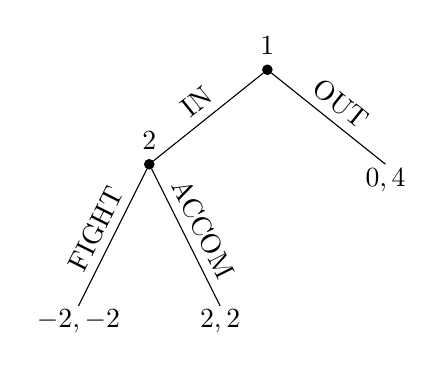
\begin{tikzpicture}[scale=1]
    % Node styles
    \tikzset{solid node/.style={circle,draw,fill=black,inner sep=1.2pt}}
    
    % --- Level 0: Root (Player 1) ---
    \node[solid node, label=above:1] (root) at (0,0) {};

    % --- Level 1 (Player 1's choices) ---
    \node[solid node, label=above:2] (n2_left) at (-1.5, -1.2) {};
    \coordinate (out) at (1.5, -1.2);

    % Edges from Root
    \draw (root) -- (n2_left) node[midway, above, sloped] {IN};
    \draw (root) -- (out) node[midway, above, sloped] {OUT};

    % --- Level 2: Terminal nodes (Player 2's choices lead here) ---
    \coordinate (fight) at (-2.4, -3);
    \coordinate (accom) at (-0.6, -3);

    % Edges from Player 2
    \draw (n2_left) -- (fight) node[midway, above, sloped] {FIGHT};
    \draw (n2_left) -- (accom) node[midway, above, sloped] {ACCOM};

    % --- Payoffs ---
    \node at (1.5, -1.4) {$0, 4$};
    \node at (-2.4, -3.2) {$-2, -2$};
    \node at (-0.6, -3.2) {$2, 2$};
\end{tikzpicture}
\end{center}

From its normal form (payoff matrix) below, we know that there are two Nash equilibria: (OUT, FIGHT) and (IN, ACCOM).

\[
\begin{array}{c|cc}
 & \text{FIGHT} & \text{ACCOM} \\
\hline
\text{OUT} & 0, 5 & 0, 5 \\
\text{IN} & -2, -2 & 2, 2
\end{array}
\]

However, only (IN, ACCOM) is a subgame perfect equilibrium, because if Player 1 chooses IN, then Player 2's best response is to choose ACCOM (so to choose FIGHT is not a credible threat). Therefore, the unique subgame perfect equilibrium is (IN, ACCOM).

Suppose now the game is repeatedly played for $T = 20$ times. 
At $t = 1$, Player 1 chooses IN or OUT. If Player 1 chooses OUT, the game ends. If Player 1 chooses IN, then in any period $t\ge 1$, the Player 1 can choose to stay (IN) or exit (OUT). If OUT is ever chosen by Player 1, then OUT for all the periods onwards.

Clearly, using backward induction, we know that the unique subgame perfect equilibrium is for Player 1 to choose IN and Player 2 to choose ACCOM in all periods.

However, if we add one additional constraint: Player 1 can only fight for at most 15 periods, then the analysis changes.

\clmp{}{
  The unique SPE with the constraint is that
  \begin{itemize}
    \item Player 1 never enters (IN), and
    \item Player 2 chooses FIGHT if Player chooses IN.
  \end{itemize}
}{
  Suppose that Player 1 has entered and been fought for the previous 14 periods. In period $t=15$, if Player 1 chooses IN, Player 2 compares the payoffs of FIGHT and ACCOM:
  \begin{itemize}
    \item If Player 2 chooses \text{FIGHT}: Player 1's capacity is exhausted, forcing them to choose OUT from $t=16$ to $t=20$. Player 2's total remaining payoff is $-2 (\text{at } t=15) + 5 \times 4 (\text{monopoly profit}) = 18$.
    \item If Player 2 chooses \text{ACCOM}: Player 1 stays in the market. Player 2's total remaining payoff is $2 (\text{at } t=15) + 5 \times 2 (\text{duopoly profit}) = 12$.
  \end{itemize}
  Since $18 > 12$, FIGHT becomes a \textit{credible threat} at $t=15$. Anticipating this, Player 1 will choose OUT at $t=15$ to avoid the $-2$ payoff.

  Consider period $t=14$. Player 1 anticipates that choosing IN will result in Player 2 choosing FIGHT (to trigger the exit at $t=15$ and secure future monopoly profits). Choosing IN at $t=14$ followed by exit at $t=15$ yields a lower payoff than choosing OUT immediately at $t=14$. 

  Following this logic backward to $t=1$, consequently, the only rational choice for Player 1 is to never enter (OUT), and for Player 2 to threaten to FIGHT at any entry node.
}

}



\thmp{}{
  Every finite game in extensive form has at least one subgame perfect equilibrium.
}{
The proof is to find all subgames that do not have any proper subgames. In each such subgame, find a Nash equilibrium of the subgame, and replace each node by expected payoffs from any Nash equilibrium of the subgame. 
}

\rmkb[]{
The notion of subgame perfect equilibrium is to generalize backward induction to games with imperfect information. 
}

\ex[Centipede Game]{

\begin{center}
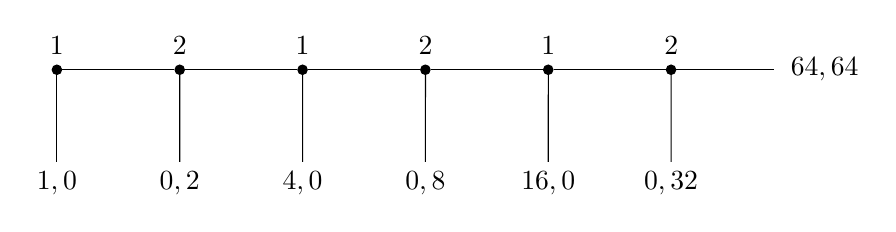
\begin{tikzpicture}[scale=1.3, font=\normalsize]
    \tikzset{solid node/.style={circle,draw,fill=black,inner sep=1.2pt}}
    
    % Main horizontal chain of nodes (closer spacing)
    \node[solid node, label=above:1] (p1_1) at (0, 0) {};
    \node[solid node, label=above:2] (p2_1) at (1.2, 0) {};
    \node[solid node, label=above:1] (p1_2) at (2.4, 0) {};
    \node[solid node, label=above:2] (p2_2) at (3.6, 0) {};
    \node[solid node, label=above:1] (p1_3) at (4.8, 0) {};
    \node[solid node, label=above:2] (p2_3) at (6, 0) {};
    \coordinate (end) at (7, 0) {};
    
    % Horizontal chain edges (no labels)
    \draw (p1_1) -- (p2_1);
    \draw (p2_1) -- (p1_2);
    \draw (p1_2) -- (p2_2);
    \draw (p2_2) -- (p1_3);
    \draw (p1_3) -- (p2_3);
    \draw (p2_3) -- (end);
    
    % Downward branches (Exit payoffs, shorter)
    \draw (p1_1) -- (0, -0.9) node[below] {$1,0$};
    \draw (p2_1) -- (1.2, -0.9) node[below] {$0,2$};
    \draw (p1_2) -- (2.4, -0.9) node[below] {$4,0$};
    \draw (p2_2) -- (3.6, -0.9) node[below] {$0,8$};
    \draw (p1_3) -- (4.8, -0.9) node[below] {$16,0$};
    \draw (p2_3) -- (6, -0.9) node[below] {$0,32$};
    
    % Final outcome (on the right)
    \node at (7.5, 0) {$64,64$};
    
\end{tikzpicture}
\end{center}

    The unique subgame perfect equilibrium is for each player to exit immediately at their first decision node, yielding payoff $(1, 0)$. However, the backward induction outcome $(1, 0)$ is Pareto dominated by the outcome $(64, 64)$ at the end. Both players would be better off if the game continued to the end, but the equilibrium logic prevents this.
}

\section{Subgame Perfection}
\ex[Selten's Horse]{

\begin{center}
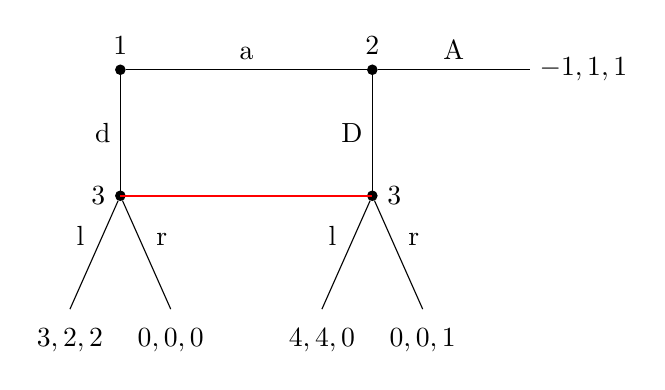
\begin{tikzpicture}[scale=0.8, font=\normalsize]
    \tikzset{solid node/.style={circle,draw,fill=black,inner sep=1.2pt}}
    
    % Level 0 - Player 1 (moved up, was p2_left)
    \node[solid node, label=above:1] (p1) at (-2, 0) {};
    
    % Level 0 - Player 2 (was p2_right)
    \node[solid node, label=above:2] (p2) at (2, 0) {};
    
    % Tree trunk connecting Player 1 and Player 2
    \draw (p1) -- (p2) node[midway, above] {a};
    
    % Level 1 - Player 3 nodes (with information set dashed line)
    \node[solid node, label=left:3] (p3_left) at (-2, -2) {};
    \node[solid node, label=right:3] (p3_right) at (2, -2) {};
    
    % Edges from Player 1 to left Player 3
    \draw (p1) -- (p3_left) node[midway, left] {d};
    
    % Edges from Player 2 to right Player 3
    \draw (p2) -- (p3_right) node[midway, left] {D};
    
    % Information set: red solid line connecting the two player 3 nodes
    \draw[red, thick] (-2, -2) -- (2, -2);
    
    % Branch from Player 2 going right to outcome
    \draw (p2) -- (4.5, 0) node[midway, above] {A} node[right] {$-1,1,1$};
    
    % Level 2 - Terminal outcomes from left Player 3
    \draw (p3_left) -- (-2.8, -3.8) node[midway, above left] {l};
    \node at (-2.8, -4.3) {$3,2,2$};
    
    \draw (p3_left) -- (-1.2, -3.8) node[midway, above right] {r};
    \node at (-1.2, -4.3) {$0,0,0$};
    
    % Level 2 - Terminal outcomes from right Player 3
    \draw (p3_right) -- (1.2, -3.8) node[midway, above left] {l};
    \node at (1.2, -4.3) {$4,4,0$};
    
    \draw (p3_right) -- (2.8, -3.8) node[midway, above right] {r};
    \node at (2.8, -4.3) {$0,0,1$};
    
\end{tikzpicture}
\end{center}

There are two pure strategy Nash equilibria: $(d, A, l)$ and $(a, A, r)$. Since this game has no proper subgames, both equilibria are subgame perfect.

However, the SPE $(d, A, l)$ appears problematic: if Player 1 accidentally chooses $a$ instead of $d$, Player 2 would prefer to choose $D$ rather than $A$. This suggests the equilibrium is not robust to small mistakes.
}

Recall that $\sigma$ is a Nash equilibrium if and only if for each player $i$ and any pure strategy $s_i'$: $u_i(\sigma_i,\sigma_{-i}) \geq u_i(s_i',\sigma_{-i})$, and for all the pure strategies that are in the support of $\sigma_i$, the expected payoff is the same: $u_i(s_i,\sigma_{-i}) = u_i(\sigma_i,\sigma_{-i})$ for all $s_i$ such that $\sigma_i(s_i) > 0$.
Hence, if for some pure strategy $s_i'$, we have $u_i(\sigma_i,\sigma_{-i}) > u_i(s_i',\sigma_{-i})$, then $\sigma_i(s_i') = 0$.

To formalize the intuition from the previous example of Selten's Horse, suppose all players' choices are subject to small trembles (mistakes).


\defn{$\varepsilon$-Equilibrium}{
  A mixed strategy profile $\sigma^{\varepsilon}$ is an \textit{$\varepsilon$-equilibrium} (for small $\varepsilon > 0$) if:
  \begin{itemize}
    \item Every pure strategy has positive probability: $\sigma_i^{\varepsilon}(s_i) > 0$ for all $i$ and $s_i$.
    \item Strategies that are not a best response are played with low probability: if $u_i(s_i',\sigma_{-i}^{\varepsilon}) > u_i(s_i,\sigma_{-i}^{\varepsilon})$, then $\sigma_i^{\varepsilon}(s_i') < \varepsilon$.
  \end{itemize}
}

\defn{Trembling Hand Perfect Equilibrium}{
  A strategy profile $\sigma$ is a \textit{trembling hand perfect equilibrium} (THPE) if it is the limit of a sequence of $\varepsilon$-equilibria $\sigma^{\varepsilon}$ as $\varepsilon \to 0$.
}

